\subsection{Euler's Method}
Euler's method is by far the simplest of the 5 explicit approximation 
methods employed in this paper. It uses the current slope at point $x_i$, ($i = 0, \dots, n)$ for n subintervals) which can be found by evaluating one of our differential equations at $f(t_i, x_i)$, We then multiply by our step size h, and add this term to our original point $x_i$ to approximate the point $x_{i+1}$. We then end up with the following formula: $$x_{i+1}=x_i+hf(t_i, x_i)$$

The error approximation for Euler's method is as follows. For an exact 
point $x_i$, it is known that the next point $x_{i+1}$ will at most have an error of $\mathcal{O}(h^2)$. However, this error can accumulate over time. After n iterations, we are left with $n*h^2 = (1/h)*h^2$, meaning our worst-case error is actually represented by $\mathcal{O}(h)$.

\subsection{Improved Euler's Method}
Improved Euler's method is similar, but lends itself to higher 
performance because it uses two different slope approximations to compute the slope at $x_i$. The first approximation, $k_1$, is simply the $f(t_i,x_i)$ computed in the basic Euler's Method. 
Then, $k_2 = hf(t_{i+1}, x_i +hk_1)$. 
This is essentially an approximation of the slope at the next point, $t_{i+1}$. 
The idea is that our look-ahead slope will correct some over/underestimation from our original slope. 
The final equation is as simple as taking a step h with the average of our two slopes: 
$$x_{i+1}=x_i+h(k_1+k_2)$$ 
For an exact $x_i$, we know $x_{i+1}$ to have an error $\mathcal{O}(h^3)$. 
However, as before, we must account for accumulated error. Thus, our final error is $\mathcal{O}(h^2)$.


\subsection{Runge-Kutta Method of Order 4 (RK4)}
The RK4 method uses a combination of 4 different slopes, and takes their weighted average to approximate the slope at $x_{i+1}$ given some $x_i$. Thus, we have $k_1$,$k_2$,$k_3$, and $k_4$ formulated as such: 

\begin{equation}
    \label{k1} k_1=f(t_i,x_i)
\end{equation}
\begin{equation}
    \label{k1} k_2=f(t_i+h/2,x_i+h/2k_1)
\end{equation}
\begin{equation}
    \label{k1} k_3=f(t_i+h/2,x_i+h/2k_2)
\end{equation}
\begin{equation}
    \label{k1} k_4=f(t_i+h,x_i+hk_3)
\end{equation}
Then, a weighted average is taken to compute the slope at $x_{i+1}$:

\begin{equation}
    \label{k1} x_{i+1}=x_i+\frac{h}{6}(k_1+2k_2+2k_3+k_4)
    \end{equation}
This can also be represented with the following Butcher tableau: 
\begin{figure}
    \centering
    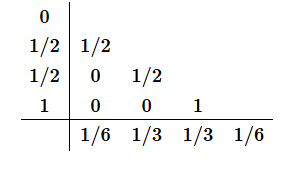
\includegraphics[width=0.5\linewidth]{Figures/rk4tab.png}
    \label{fig:placeholder}
\end{figure}

Whereas the bottom section gives coefficients for each $k_i$, the left section gives the coefficents of h to be added to $t_i$ for each $k_i$, and the diagonal gives coefficents of each h to be multiplied by the corresponding $k_i$ and then subsequently to be added to $t_i$, for each $k_i$. As the name suggests, the error of this method is of order $\mathcal{O}(h^4)$.


\subsection{Runge–Kutta–Fehlberg 45 Adaptive Method (RKF45)}
This adaptive method uses the following Butcher tableau:



\begin{figure}
    \centering
    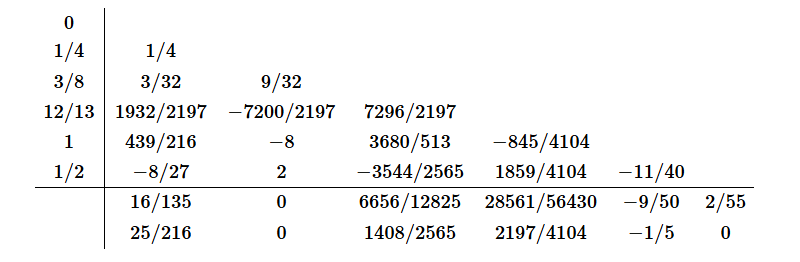
\includegraphics[width=\linewidth]{Figures/rkf45tab.png}
\end{figure}

Whereas the second row produces a method of fifth-order accuracy, while the first produces a method of fourth-order accuracy. At each step, we compute $x_{i+1}$ using both methods, which requires 6 evaluations of $f$. If they produce a difference (an error) outside of our prescribed tolerance, we halve the step size and continue to $x_{i+1}$. 
In addition to an error tolerance, we provide a minimum and maximum h. When we go below the minimum h, we do not halve the h, even if our error tolerance has not been reached. Instead, the method flags the failure and adds it to a tally.  While we are still using an $\mathcal{O}(h^4)$ method, we now dynamically adjust the step size, hopefully resulting in less overall computation to achieve the same error. 

\subsection{Dormand–Prince 45 Adaptive Method (DP45)}
This adaptive method uses the following Butcher tableau:
\begin{figure}
    \centering
    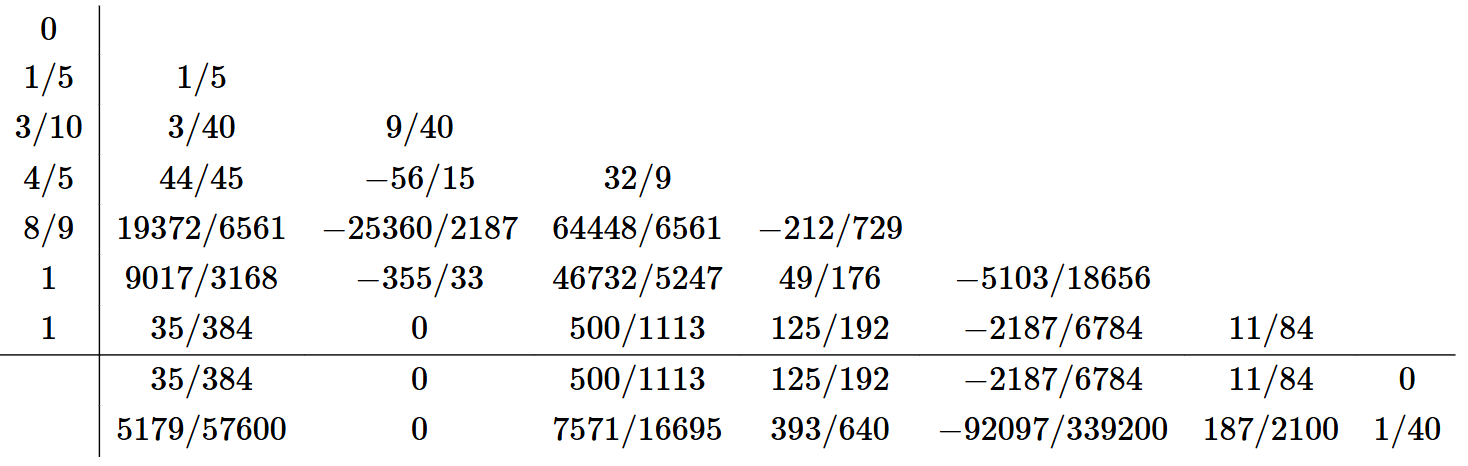
\includegraphics[width=\linewidth]{Figures/dp45tab.png}
\end{figure}

Again, the second row produces a method of fifth-order accuracy, while the first produces a method of fourth-order accuracy. The adaptive aspect of the method works just as in RKF45. Note that the same coefficients are used to compute $k_7$ as are used to compute the fourth-order estimation; this means that this method requires 6 evaluations of $f$ per step, like RKF45. 

\subsection{Determination of a Reference Solution}
Exact solutions cannot be determined analytically for the given system of ODEs, so a method was proposed to compare the error with results from a low-tolerance RKF45 approximation using model parameters from Table ~\ref{tab:constants}. Tolerances for the reference solution are defined within $10^{-16}$ to $10^{-14}$. Comparison to the same model with tolerances between $10^{-12}$ to $10^{-10}$ yields a close idea of reference convergence to the exact solution. Absolute errors between the two tolerances for both species are shown in Figure ~\ref{fig:errordifference}. 

As shown, all errors are $<10^{-9}$, so we consider the reference to approximate the exact solution well. Understanding this limitation, we target an error for all numerical conditions on the order of $10^{-2}$ to ensure the scale of error between our reference and the exact solution does not meaningfully interfere with the calculated error for each method and the reference.

\begin{figure}[!h]
    \centering
    % Adjust [width=0.8\textwidth] if you want it larger or smaller on the page
    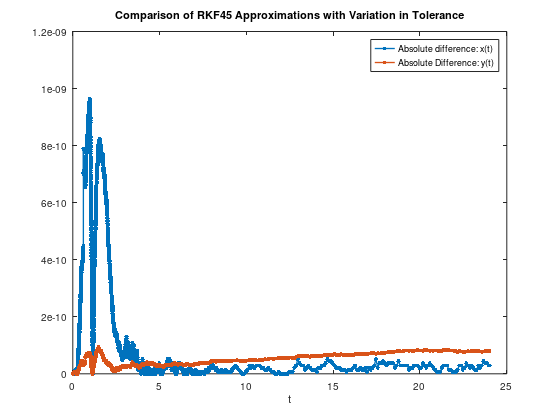
\includegraphics[width=1.0\textwidth, height=0.85\textheight, keepaspectratio]{Figures/errordifference.png}
    \caption{Absolute errors between RKF45 approximations with tolerances between $10^{-16}$ and $10^{-14}$ (reference) and tolerances between $10^{-12}$ and $10^{-10}$.}
    \label{fig:errordifference}
\end{figure}

As RKF45 involves variable step sizes, interpolation is required to calculate the error between methods. 
The reference equation is interpolated using the Octave interp1() function, using a spline method. 
From here, calculating maximum absolute error is as simple as finding the maximum absolute difference between the solution vectors for each population density.